% ==============================================================================
% Design Education in Ukraine: Competency Development and European Integration
% in Artistic-Project Training of Future Design Professionals
% 
% Paper Type: Theoretical Paper (Document/Policy Analysis)
% ==============================================================================

\documentclass[ed]{acnsart}

\setdoi{10.31812/ed.1112}
\setjournalyear{2025}
\setjournalvolume{13}
%\setjournalissue{4}
\setcounter{page}{257}

% ==============================================================================
% TABLES
% ==============================================================================
\usepackage{booktabs}
\usepackage{tabularx}
\usepackage{longtable}
\usepackage{multirow}
\usepackage{array}

% ==============================================================================
% FIGURES AND GRAPHICS
% ==============================================================================
\usepackage{tikz}
\usepackage{pgfplots}
\pgfplotsset{compat=1.18}
\usetikzlibrary{shapes, arrows, positioning, calc, mindmap, trees, shadows, decorations.pathreplacing, fit, backgrounds}
\usepackage{graphicx}
\usepackage{float}

% ==============================================================================
% TYPOGRAPHY AND FORMATTING
% ==============================================================================
%\usepackage{microtype}
\usepackage{enumitem}
\usepackage{csquotes}


% ==============================================================================
% BEGIN DOCUMENT
% ==============================================================================
\begin{document}
	% ==============================================================================
	% TITLE AND AUTHOR
	% ==============================================================================
	\title{Design education in Ukraine: competency development and European integration in artistic-project training of future design professionals}
	
	\author{Oleksandr O. Musiienko}[
	email={musyaleksandr1110@gmail.com},
	url={https://kdpu.edu.ua/personal/musienko12911.html},
	orcid={0000-0003-4906-8172}
	] 
	
	\address{Kryvyi Rih State Pedagogical University, 54 Universytetskyi Ave., Kryvyi Rih, 50086, Ukraine}
	
	
	
	
	% Include Abstract
	% ==============================================================================
	% SECTION 1: ABSTRACT
	% Design Education in Ukraine: Competency Development and European Integration
	% ==============================================================================
	
	\begin{abstract}
Design education occupies a distinctive position at the intersection of artistic creativity and technical proficiency, presenting unique challenges for competency-based curriculum development. As Ukraine continues its integration into the European Higher Education Area following its 2005 accession to the Bologna Process, design education programs face the imperative of aligning national standards with European competency frameworks while preserving the distinctive pedagogical traditions of artistic-project training. The Ukrainian higher education standard B2 Design establishes competency requirements for design professionals, yet the theoretical foundations connecting these requirements to European frameworks and effective pedagogical approaches remain underdeveloped. This theoretical paper examines the conceptual foundations of design education competency development within the context of Ukrainian European integration. It addresses three interrelated questions: (1) How do the competency structures embedded in Ukraine's B2 Design standard correspond to European qualification frameworks and international design education models? (2) What pedagogical approaches offer the strongest theoretical grounding for developing artistic-project competencies in design students? (3) What conceptual considerations emerge from analysing European integration challenges and opportunities for Ukrainian design education? The study employs a theoretical analysis approach, synthesising international scholarship on design education, competency-based learning, and European higher education policy. Through a systematic analysis of the Ukrainian B2 Design standard and a comparative examination of European competency frameworks, the paper develops an integrative conceptual model for understanding the development of design education competencies. The analysis draws on reflective practice theory, constructive alignment principles, and design cognition research to establish theoretical foundations for enhancing the curriculum. The analysis reveals three principal insights. First, while the Ukrainian design standard demonstrates structural alignment with the European Qualifications Framework's tripartite categorisation of knowledge, skills, and competence, significant gaps exist in articulating design-specific competencies related to critical reflection, interdisciplinary collaboration, and sustainable design practices. Second, studio-based and project-based pedagogical approaches, when grounded in reflective practice theory, provide robust frameworks for developing the integrated competencies required for professional design practice. Third, European integration presents both challenges~-- including resource constraints, faculty development needs, and assessment harmonisation~-- and opportunities for curriculum innovation, international collaboration, and enhanced graduate mobility. The paper contributes a theoretically grounded framework for understanding competency development in design education within the European integration context. It proposes that effective design education reform requires simultaneous attention to three interconnected dimensions: alignment with international competency frameworks, adoption of pedagogically sound approaches to artistic-project training, and strategic engagement with European integration mechanisms. The framework offers implications for design educators, curriculum developers, and policymakers in Ukraine and other countries navigating similar integration trajectories. Future research directions include empirical validation of the proposed model and comparative studies across post-Soviet design education systems.
	\end{abstract}
	
	\begin{keywords}
		design education \sep
		competency-based learning \sep
		European integration \sep
		artistic-project activity \sep
		higher education reform \sep
		Ukraine \sep
		curriculum development
	\end{keywords}
	
	% ==============================================================================
	% END OF ABSTRACT SECTION
	% ==============================================================================
	
	\maketitle
	
	% Include Introduction
	% ==============================================================================
	% SECTION 2: INTRODUCTION
	% Design Education in Ukraine: Competency Development and European Integration
	% ==============================================================================
	
	\section{Introduction}
	
	Design has emerged as one of the defining professional disciplines of the twenty-first century, shaping not merely the aesthetic dimensions of material culture but increasingly the complex systems, services, and experiences that structure contemporary life \cite{Davis202397}. As the scope of design practice expands from the production of tangible artefacts to the stewardship of evolving product-service ecologies, design education faces the imperative of preparing professionals capable of navigating unprecedented complexity while maintaining the creative and aesthetic sensibilities that distinguish design from other problem-solving disciplines \cite{Maia2022105}. This transformation demands fundamental reconsideration of how design competencies are conceptualised, developed, and assessed within higher education.
	
	The challenges confronting design education are amplified for countries undergoing simultaneous processes of educational reform and regional integration. Ukraine presents a particularly instructive case: having acceded to the Bologna Process in 2005 at the Bergen Conference, the country committed to harmonising its higher education system with European norms while preserving the distinctive traditions of artistic-technical training inherited from Soviet-era institutions \cite{Fursa2014}. The Ukrainian higher education standard 022 (B2) Design, established by the Ministry of Education and Science in 2018, represents an attempt to articulate competency requirements consonant with European frameworks while addressing the specific needs of the national design profession and labour market \cite{MON2018}. However, significant questions remain regarding the theoretical foundations of this standard, its alignment with international best practices, and the pedagogical approaches best suited to realising its competency objectives.
	
	The contemporary design educator confronts what \citet{Maia2022105} characterises as a profession under pressure to evolve towards increasingly complex activity requiring new general and specialised skills. The design community recognises the value of multidisciplinary capabilities and the ability to lead processes involving large socio-technical systems. However, designers must increasingly operate within multidisciplinary teams where required competencies extend far beyond traditional artistic and technical abilities. This tension between disciplinary distinctiveness and interdisciplinary integration poses particular challenges for curriculum design and pedagogical practice. Moreover, emerging technologies~-- including artificial intelligence, virtual and augmented reality, and generative design tools~-- are introducing additional layers of complexity into design education, requiring educators to balance technological fluency with foundational design capabilities \cite{Chen2025, Song2025401}.
	
	Within this context of rapid transformation, competency-based approaches to curriculum development have gained prominence across European higher education following the Bologna Process reforms \cite{Castillo2011230}. The European Qualifications Framework establishes a tripartite categorisation of learning outcomes~-- knowledge, skills, and competence~-- that has become normative for curriculum design across the European Higher Education Area. However, the application of these frameworks to creative disciplines such as design raises distinctive challenges, particularly regarding the assessment of tacit knowledge, the development of aesthetic judgement, and the cultivation of creative capabilities that resist standardised measurement \cite{Gehmlich2009736}. The studio-based pedagogies central to design education operate according to logics that may not align straightforwardly with competency-based frameworks, creating tensions that curriculum developers must navigate \cite{Mewburn2012363, Goldschmidt2010285}.
	
	Ukrainian design education, emerging from a tradition that emphasised artistic-constructive training within specialised academies, faces the particular challenge of integrating European competency frameworks without sacrificing the strengths of established pedagogical approaches. The B2 Design standard identifies both general and professional competencies required for design graduates, establishing learning outcomes oriented toward preparing specialists capable of solving complex design problems in conditions of incomplete information while demonstrating creativity and innovation. However, the conceptual foundations connecting these competency requirements to effective pedagogical approaches remain underdeveloped in Ukrainian scholarship, which has tended toward descriptive rather than analytical treatment of design education development \cite{Fursa2014}.
	
	This theoretical paper addresses this gap by examining the conceptual foundations of design education competency development within the context of Ukrainian European integration. Three interrelated research questions guide the analysis:
	
	\begin{enumerate}[label=\textbf{RQ\arabic*:}, leftmargin=*]
		\item How do the competency structures embedded in Ukraine's B2 Design standard correspond to European qualification frameworks and international design education models?
		\item What pedagogical approaches offer the strongest theoretical grounding for developing artistic-project competencies in design students?
		\item What conceptual considerations emerge from analysing European integration challenges and opportunities for Ukrainian design education?
	\end{enumerate}
	
	These questions reflect an understanding that effective design education reform requires attention to multiple interconnected dimensions: the formal structures of competency frameworks, the pedagogical practices through which competencies are developed, and the broader policy contexts within which educational institutions operate. Figure~\ref{fig:conceptual-framework} presents the conceptual relationships among these dimensions that structure the analysis.
	
	\begin{figure}[htbp]
		\centering
		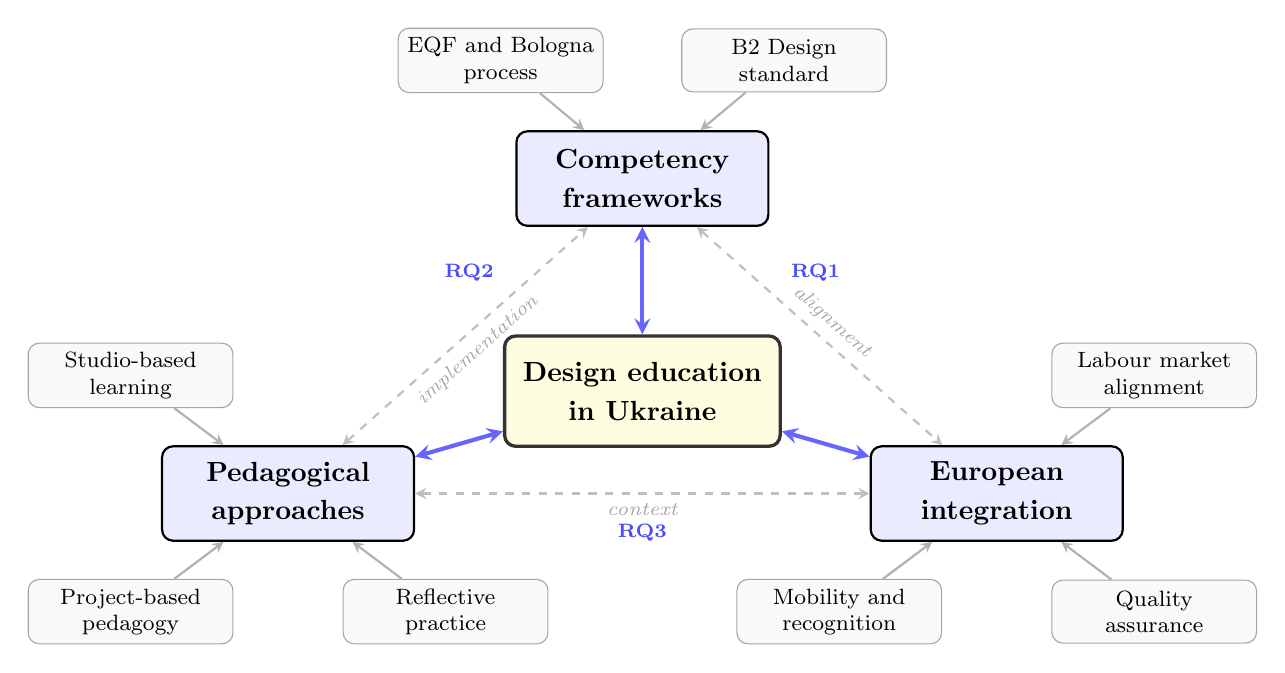
\begin{tikzpicture}[
			% Define styles
			mainbox/.style={rectangle, draw=black, thick, rounded corners, minimum width=3.2cm, minimum height=1.2cm, align=center, fill=blue!8},
			subbox/.style={rectangle, draw=gray!70, rounded corners, minimum width=2.6cm, minimum height=0.8cm, align=center, fill=gray!5, font=\footnotesize},
			connector/.style={->, thick, >=stealth, draw=black!70},
			bidirectional/.style={<->, thick, >=stealth, draw=black!70},
			label/.style={font=\scriptsize\itshape, text=gray!70}
			]
			
			% Main nodes - triangular arrangement
			\node[mainbox] (competency) at (0,4) {\textbf{Competency}\\[2pt]\textbf{frameworks}};
			\node[mainbox] (pedagogy) at (-4.5,0) {\textbf{Pedagogical}\\[2pt]\textbf{approaches}};
			\node[mainbox] (integration) at (4.5,0) {\textbf{European}\\[2pt]\textbf{integration}};
			
			% Central node
			\node[rectangle, draw=black!80, very thick, rounded corners, minimum width=3.5cm, minimum height=1.4cm, align=center, fill=yellow!12] (design) at (0,1.3) {\textbf{Design education}\\[2pt]\textbf{in Ukraine}};
			
			% Sub-nodes for Competency Frameworks
			\node[subbox] (eqf) at (-1.8,5.5) {EQF and Bologna\\process};
			\node[subbox] (standard) at (1.8,5.5) {B2 Design\\standard};
			
			% Sub-nodes for Pedagogical Approaches
			\node[subbox] (studio) at (-6.5,1.5) {Studio-based\\learning};
			\node[subbox] (project) at (-6.5,-1.5) {Project-based\\pedagogy};
			\node[subbox] (reflective) at (-2.5,-1.5) {Reflective\\practice};
			
			% Sub-nodes for European Integration
			\node[subbox] (mobility) at (2.5,-1.5) {Mobility and \\recognition};
			\node[subbox] (quality) at (6.5,-1.5) {Quality\\assurance};
			\node[subbox] (labour) at (6.5,1.5) {Labour market\\alignment};
			
			% Connections from sub-nodes to main nodes
			\draw[connector, gray!60] (eqf) -- (competency);
			\draw[connector, gray!60] (standard) -- (competency);
			\draw[connector, gray!60] (studio) -- (pedagogy);
			\draw[connector, gray!60] (project) -- (pedagogy);
			\draw[connector, gray!60] (reflective) -- (pedagogy);
			\draw[connector, gray!60] (mobility) -- (integration);
			\draw[connector, gray!60] (quality) -- (integration);
			\draw[connector, gray!60] (labour) -- (integration);
			
			% Main bidirectional connections
			\draw[bidirectional, blue!60, line width=1.5pt] (competency) -- (design);
			\draw[bidirectional, blue!60, line width=1.5pt] (pedagogy) -- (design);
			\draw[bidirectional, blue!60, line width=1.5pt] (integration) -- (design);
			
			% Inter-dimension connections (dashed)
			\draw[bidirectional, dashed, gray!50] (competency) -- node[label, above, sloped] {alignment} (integration);
			\draw[bidirectional, dashed, gray!50] (pedagogy) -- node[label, below, sloped] {implementation} (competency);
			\draw[bidirectional, dashed, gray!50] (pedagogy) -- node[label, below, sloped] {context} (integration);
			
			% Research question labels
			\node[font=\scriptsize\bfseries, text=blue!70] at (-2.2,2.8) {RQ2};
			\node[font=\scriptsize\bfseries, text=blue!70] at (2.2,2.8) {RQ1};
			\node[font=\scriptsize\bfseries, text=blue!70] at (0,-0.5) {RQ3};
			
		\end{tikzpicture}
		\caption{Conceptual framework -- three dimensions of design education development in the European integration context. The framework illustrates the interconnections among competency frameworks (RQ1), pedagogical approaches (RQ2), and European integration processes (RQ3) that together shape design education reform in Ukraine.}
		\label{fig:conceptual-framework}
	\end{figure}
	
	The paper employs a theoretical analysis approach, synthesising international scholarship on design education, competency-based learning, and European higher education policy. Through a systematic examination of the Ukrainian B2 Design standard alongside European competency frameworks, this analysis develops an integrative conceptual model for understanding the development of design education competency. The theoretical foundations draw on reflective practice theory as articulated by \citet{Schon1983}, constructive alignment principles \cite{Biggs1996}, and design cognition research \cite{Cross2011, Lawson2005}. This approach enables rigorous examination of conceptual relationships while acknowledging the limitations inherent in theoretical analysis that await empirical validation.
	
	The paper is structured as follows. Section~\ref{sec:literature} reviews international literature on design education, examining theoretical foundations, pedagogical approaches, competency frameworks, and the specific context of design education in post-Soviet and European settings. Section~\ref{sec:framework} presents the theoretical framework guiding the analysis, integrating perspectives from competency-based education, reflective practice, and design cognition. Section~\ref{sec:methodology} details the methodological approach to theoretical analysis and document examination. Section~\ref{sec:findings} presents findings organised around the three research questions, examining competency alignment, pedagogical foundations, and integration challenges. Section~\ref{sec:discussion} interprets these findings in relation to existing scholarship and develops implications for theory and practice. Section~\ref{sec:conclusion} summarises contributions and identifies directions for future research.
	
	This paper contributes to design education scholarship in three principal ways. First, it provides a systematic analysis of Ukrainian design education standards in relation to European frameworks, addressing a gap in English-language literature on post-Soviet design education reform. Second, it develops a theoretically grounded framework for understanding competency development in design education that integrates European policy frameworks with pedagogical theory. Third, it provides conceptual resources for design educators and policymakers navigating similar integration trajectories, with implications extending beyond the Ukrainian context to other countries that are engaging with European higher education harmonisation while maintaining their distinctive educational traditions.
	
	% ==============================================================================
	% END OF INTRODUCTION SECTION
	% ==============================================================================
	
	% Include Literature Review
	% ==============================================================================
	% SECTION 3: LITERATURE REVIEW
	% Design Education in Ukraine: Competency Development and European Integration
	% ==============================================================================
	
	\section{Literature review}
	\label{sec:literature}
	
	This section reviews international scholarship on design education, organised thematically to establish the conceptual foundations for the subsequent analysis. The review examines theoretical underpinnings of design education, pedagogical approaches, competency-based frameworks, and the specific contexts of European and post-Soviet design education development.
	
	\subsection{Design education: conceptual foundations and historical development}
	
	Design education occupies a distinctive epistemological position, integrating artistic creativity with technical rationality in ways that distinguish it from both fine arts and engineering disciplines \cite{Cross2018691}. The field has developed what \citet{Oxman1999105} terms `designerly thinking'~-- cognitive structures and strategies specific to design practice that require explicit pedagogical attention. Understanding these foundations is essential for analysing contemporary competency frameworks and their implementation.
	
	The historical development of formalised design education is conventionally traced to the Bauhaus school (1919--1933), whose pedagogical innovations continue to influence contemporary practice \cite{Sturgis20209, Aynsley2022209}. The Bauhaus Basic Course, developed by Johannes Itten and subsequently modified by László Moholy-Nagy and Josef Albers, established foundational principles that included the integration of craft and industrial production, systematic colour and form studies, and an emphasis on learning through making \cite{Cross198343}. \citet{Sinico202199} demonstrates the influence of Gestalt psychology on Bauhaus pedagogy, revealing how Walter Gropius's educational philosophy incorporated phenomenological attitudes as fundamental to design practice. These foundations~-- the integration of artistic and technical knowledge, experiential learning, and systematic skill development~-- remain embedded in contemporary design curricula globally.
	
	The post-Bauhaus evolution of design education proceeded through several significant phases. The Ulm School of Design (1953--1968) introduced more systematic, scientifically-grounded approaches to design methodology, emphasising research and rational problem-solving \cite{Li2023}. The subsequent emergence of design thinking as both a professional methodology and an educational framework marks another paradigmatic shift, extending design approaches beyond traditional design disciplines into management, innovation, and social problem-solving \cite{Razzouk2012330}. \citet{Davis202397} argues that contemporary design education must now address a fundamental paradigm shift from twentieth-century artefact production to twenty-first-century stewardship of complex product-service ecologies.
	
	The conceptualisation of design cognition has been substantially developed through empirical research on expert designers. \citet{Cross2018691} synthesises fifty years of design research, articulating the concept of `designerly ways of knowing' and establishing design as a legitimate discipline with distinctive epistemological characteristics. This research demonstrates that expert designers exhibit characteristic cognitive patterns, including the co-evolution of problem and solution, abductive reasoning, and iterative refinement through prototyping \cite{Kokotovich200849, Atman2019125}. \citet{Haupt2015483} extends this understanding through the lens of extended cognition theory, arguing that design thinking operates by coupling internal cognitive processes with external resources and representations.
	
	The implications for design education are significant: effective pedagogy must develop not merely technical skills and aesthetic sensibilities but the specific cognitive dispositions characteristic of expert design practice. \citet{Chon2019187} distinguishes between design thinking (procedural knowledge) and design knowing (conceptual understanding), arguing that design education must cultivate both dimensions through carefully structured pedagogical experiences.
	
	\subsection{Pedagogical approaches in design education}
	
	The design studio remains the signature pedagogical environment in design education, distinguished by its integration of individual creative work, collaborative learning, and expert mentorship \cite{Goldschmidt2010285}. Studio-based learning embodies what \citet{Schon1983} characterises as reflective practice~-- the capacity for reflection-in-action through which practitioners develop expertise in handling complex, ill-defined problems. \citet{Mewburn2012363} offers a performative account of studio pedagogy, demonstrating how knowledge is produced through complex interactions among students, teachers, and design artefacts.
	
	The desk critique (`crit') constitutes the primary instructional interaction within studio pedagogy, enabling one-on-one dialogue between student and instructor regarding work in progress \cite{Goldschmidt2010285}. \citet{Ardington2017157} analyses the discourse of design studio assessment, revealing tensions between the need for explicit guidance and the preservation of creative freedom essential to design learning. The subjective nature of design assessment, negotiated through discourse grounded in tacit disciplinary understandings, presents ongoing challenges for competency-based frameworks that require explicit articulation of learning outcomes.
	
	Project-based learning complements studio pedagogy by situating design challenges within authentic professional contexts \cite{Kamalipour2022}. Effective project-based approaches enable students to develop integrated competencies through engagement with complex, open-ended problems that resist formulaic solutions \cite{Tsai2023}. \citet{Sung2019283} identifies that idea generation plays a central role in design processes, with iterative patterns characterising expert practice. These insights inform curriculum design by emphasising the importance of extended project engagement and iterative development cycles.
	
	The integration of reflective practice within design education has received substantial theoretical and empirical attention. \citet{Hameed2023310} demonstrates that digital reflective practice in textile design education enhances creativity through enabling revisitation and reconstruction of design work. This aligns with \citeauthor{Schon1983}'s \cite{Schon1983} foundational argument that professional expertise develops through systematic reflection on action. Contemporary approaches increasingly emphasise metacognitive development alongside technical skill acquisition \cite{Yusuf2026}.
	
	Table~\ref{tab:pedagogical-approaches} summarises the principal pedagogical approaches in design education and their characteristic features.
	
	\begin{table}[htbp]
		\centering
		\caption{Principal pedagogical approaches in design education.}
		\label{tab:pedagogical-approaches}
		\small
		\begin{tabularx}{\textwidth}{@{}p{2.8cm}Xp{4.2cm}@{}}
			\toprule
			\hfil \textbf{Approach} & \hfil \textbf{Key characteristics} & \hfil \textbf{Primary sources} \\
			\midrule
			Studio-based learning & Individual workspace; desk critiques; master-apprentice relationships; learning through making; peer observation & \citet{Schon1983}; \citet{Goldschmidt2010285}; \citet{Mewburn2012363} \\
			\addlinespace
			Project-based learning & Authentic design briefs; extended engagement; iterative development; client interaction; integrated assessment & \citet{Kamalipour2022}; \citet{Tsai2023} \\
			\addlinespace
			Reflective practice & Reflection-in-action; documentation of process; metacognitive development; portfolio assessment & \citet{Schon1983}; \citet{Hameed2023310} \\
			\addlinespace
			Design thinking methodology & Empathy-driven; iterative prototyping; divergent-convergent cycles; interdisciplinary application & \citet{Razzouk2012330}; \citet{Chon2019187} \\
			\addlinespace
			Experiential learning & Learning by doing; concrete experience; reflective observation; abstract conceptualisation; active experimentation & \citet{Kolb1984}; \citet{Duchatelet2024400} \\
			\bottomrule
		\end{tabularx}
	\end{table}
	
	\subsection{Competency-based approaches in design education}
	
	Competency-based education has emerged as the dominant framework for curriculum development across European higher education following the Bologna Process reforms \cite{Castillo2011230}. The European Qualifications Framework (EQF) establishes a tripartite categorisation of learning outcomes~-- knowledge, skills, and competence~-- that provides common reference points for qualification levels across national systems \cite{Bohlinger2012279}. However, the application of these frameworks to creative disciplines raises distinctive challenges regarding the articulation and assessment of competencies that encompass tacit knowledge, aesthetic judgement, and creative capability.
	
	\citet{Gehmlich2009736} analyses the conceptual distinctions between learning outcomes and competence (`Kompetenz') in the German context, noting that competence encompasses the proven ability to apply knowledge and skills in work or study situations, including responsibility and autonomy dimensions. This definition emphasises demonstrated capability in authentic contexts rather than isolated skill performance. For design education, this implies that competency development requires engagement with genuine design challenges rather than decontextualised exercises.
	
	The tension between standardisation and creativity presents particular challenges for design education \cite{Weldon2009168}. \citet{Brockmann200899} argues that performance-based learning outcomes contain inherent design flaws when applied without consideration of the conditions and contexts in which competency is demonstrated. In design education, where creative originality is valued alongside technical proficiency, assessment frameworks must accommodate variation and novelty rather than conformity to predetermined standards.
	
	\citet{AlvarezIcaza2024} addresses the assessment of creative behaviour in higher education, distinguishing between objective performance profiles and subjective self-perception. Their research with students in design, architecture, and communication programmes reveals that design students demonstrate distinctive creative behaviour patterns, though significant individual variation exists. This underscores the importance of assessment approaches that capture individual creative development rather than applying uniform benchmarks.
	
	Table~\ref{tab:competency-frameworks} presents a comparative overview of competency frameworks relevant to design education.
	
	\begin{table}[htbp]
		\centering
		\caption{Competency frameworks relevant to design education: A comparative overview.}
		\label{tab:competency-frameworks}
		\small
		\begin{tabularx}{\textwidth}{@{}p{3.2cm}p{2.5cm}Xp{3.6cm}@{}}
			\toprule
			\hfil \textbf{Framework} & \hfil \textbf{Scope} & \hfil \textbf{Key components} & \hfil \textbf{Design applicability} \\
			\midrule
			European Qualifications Framework (EQF) & Pan-European reference & Knowledge, skills, competence (responsibility \& autonomy); 8 levels & General framework; requires disciplinary specification \\
			\addlinespace
			Tuning Project & European HE sectors & Subject-specific and generic competencies; learning outcomes approach & Applied to various disciplines; limited design-specific development \\
			\addlinespace
			National Qualifications Frameworks & National systems & Country-specific adaptations of EQF principles; varying terminology & Variable; Ukraine B2 Design as example \\
			\addlinespace
			Professional Body Standards & Disciplinary & Practice-oriented competencies; accreditation requirements & Design councils and professional associations \\
			\addlinespace
			21st Century Skills Frameworks & General education & Creativity, critical thinking, collaboration, communication & Highly relevant but non-specific \\
			\bottomrule
		\end{tabularx}
	\end{table}
	
	\subsection{Design education in the European context}
	
	The Bologna Process has profoundly influenced design education across Europe, establishing common degree structures, credit systems, and quality assurance mechanisms \cite{Castillo2011230}. The shift to learning outcomes and competency-based curricula represents not merely technical reform but fundamental reconceptualisation of educational purposes and processes. \citet{Bohlinger2012279} questions whether the development of qualifications frameworks has yielded anticipated benefits, noting implementation challenges and conceptual ambiguities that persist across European education systems.
	
	European design education exhibits considerable diversity, reflecting national traditions, institutional cultures, and disciplinary orientations. Nordic countries have developed distinctive approaches emphasising sustainability, social responsibility, and democratic design values \cite{Maia2022105}. The UK system, shaped by polytechnic traditions and subsequent university integration, emphasises professional preparation and industry engagement. Continental European traditions maintain stronger connections to fine arts and craft heritage, though increasing professionalisation has shifted many programmes toward industry-oriented competency development.
	
	The integration of emerging technologies into design education represents a significant contemporary challenge across European institutions \cite{Chen2025}. \citet{Song2025401} documents the rapid shift from general AI to generative AI applications in design education, with image generation becoming the most prevalent technology. This technological transformation requires curriculum adaptation while raising questions about the nature of design creativity and the competencies that distinguish human designers. \citet{Hwang2025239} argues that design education in the generative AI era requires fundamentally different educational goals, emphasising AI visual literacy and the role of designers as content creators combining science, art, and technology.
	
	Quality assurance mechanisms in European design education increasingly emphasise learning outcomes assessment and graduate employability \cite{Srivastava2024305}. Work-integrated learning has gained prominence as a strategy for developing employability competencies while maintaining connections between academic study and professional practice. However, tensions persist between the open-ended, exploratory nature of design education and the specification requirements of competency-based quality assurance frameworks.
	
	\subsection{Design education in post-Soviet and Ukrainian context}
	
	Design education in post-Soviet countries developed within distinctive historical circumstances, emerging from traditions that emphasised technical training within specialised academies separated from fine arts institutions \cite{Fursa2014}. The Soviet model prioritised industrial application and collective production values, with aesthetic considerations subordinated to functional and ideological requirements. This legacy continues to influence institutional structures, faculty expertise, and pedagogical traditions in contemporary design education across the region.
	
	Ukraine's accession to the Bologna Process in 2005 initiated a systematic reform of higher education, including the design of programmes. The establishment of the B2 Design standard in 2018 represents a significant milestone, articulating competency requirements aligned with European frameworks while addressing national labour market needs \cite{MON2018}. The standard identifies both general competencies (critical thinking, communication, teamwork) and professional competencies specific to design practice (artistic-project activity, aesthetic analysis, technical implementation).
	
	However, several challenges complicate the reform process. Faculty development represents a significant concern, as many design educators were trained within Soviet-era traditions and may lack familiarity with competency-based approaches and contemporary international design practices. Resource constraints limit access to current technologies and international exchange opportunities. The ongoing conflict has further disrupted educational continuity, displacing both students and faculty.
	
	Despite these challenges, Ukrainian design education demonstrates significant dynamism. Integration with European networks has expanded opportunities for student and faculty mobility. Curriculum reform has introduced contemporary approaches, including design thinking methodologies and digital design technologies. The B2 Design standard provides a framework for systematic competency development, though implementation varies across institutions.
	
	\subsection{Research gap and study rationale}
	
	The reviewed literature reveals several gaps that this study aims to address. First, while substantial scholarship examines design education in Western European and North American contexts, there is limited English-language research addressing the development of design education in post-Soviet countries, specifically in Ukraine. This geographical gap limits understanding of how design education reform proceeds in contexts of simultaneous educational transformation and European integration.
	
	Second, theoretical connections between European competency frameworks and design-specific pedagogical approaches remain underdeveloped. The literature offers rich accounts of studio-based and project-based pedagogies, and separate literature addresses competency-based curriculum development, but systematic analysis integrating these perspectives is limited. This conceptual gap hinders the development of coherent curriculum designs that meet competency framework requirements while maintaining pedagogical approaches suitable for design-based learning.
	
	Third, the specific challenges and opportunities of European integration for design education in transition countries receive limited analytical attention. While policy documents address the implementation of the Bologna Process generally, scholarly analysis of how creative disciplines navigate integration processes~-- balancing international harmonisation with distinctive national and disciplinary traditions~-- remains sparse.
	
	This study addresses these gaps through a theoretical analysis of Ukrainian design education standards in relation to European frameworks and international scholarship on design education. By developing an integrative conceptual framework that connects competency structures, pedagogical approaches, and integration processes, the analysis contributes to understanding design education reform in contexts of transition, while offering resources applicable to similar cases internationally.
	
	% ==============================================================================
	% END OF LITERATURE REVIEW SECTION
	% ==============================================================================
	
	% Include Theoretical Framework
	% ==============================================================================
	% SECTION 4: THEORETICAL FRAMEWORK
	% Design Education in Ukraine: Competency Development and European Integration
	% ==============================================================================
	
	\section{Theoretical framework}
	\label{sec:framework}
	
	This section presents the theoretical framework guiding the analysis, integrating perspectives from reflective practice theory, constructive alignment, design cognition research, and competency-based education. The framework provides conceptual resources for examining how competency structures, pedagogical approaches, and integration processes interact in design education contexts.
	
	\subsection{Integrative theoretical foundations}
	
	The theoretical framework synthesises three complementary perspectives that together illuminate the multidimensional nature of design education competency development. First, \citeauthor{Schon1983}'s \cite{Schon1983} theory of reflective practice provides a foundational understanding of how professional expertise develops through cycles of action and reflection. \citeauthor{Schon1983}'s analysis of design as a paradigmatic example of reflection-in-action establishes that design competence cannot be reduced to technical rationality but requires cultivation of capacities for dealing with unique, uncertain situations through ongoing dialogue with materials and contexts. This theoretical lens emphasises the developmental nature of design expertise and the importance of pedagogical environments that support reflective engagement.
	
	Second, \citeauthor{Biggs1996}'s \cite{Biggs1996} principle of constructive alignment offers a framework for understanding relationships between intended learning outcomes, teaching and learning activities, and assessment practices. Constructive alignment posits that effective education requires coherence among these elements: what students are expected to learn (outcomes), how they are taught (activities), and how their learning is evaluated (assessment). Applied to design education, this principle illuminates potential misalignments between competency framework specifications and studio-based pedagogies, where learning outcomes may be tacit and assessment inherently interpretive.
	
	Third, design cognition research, particularly the work of \citet{Cross2011} and \citet{Lawson2005}, provides discipline-specific theoretical grounding. \citeauthor{Cross2011}'s concept of `designerly ways of knowing' establishes design as a distinct cognitive domain, characterised by characteristic modes of reasoning, including abductive inference, solution-focused problem-solving, and the co-evolution of problem and solution. \citeauthor{Lawson2005}'s analysis of design expertise development demonstrates that expert designers exhibit qualitatively different cognitive patterns than novices, with implications for how educational programmes should structure learning progressions.
	
	\subsection{Framework architecture}
	
	Figure~\ref{fig:theoretical-framework} presents the integrative theoretical framework developed for this analysis. The framework positions design education competency development at the intersection of three interacting systems: the competency specification system (formal frameworks and standards), the pedagogical system (teaching and learning approaches), and the integration system (European harmonisation processes and quality assurance mechanisms).
	
	\begin{figure}[htbp]
		\centering
		\resizebox{\linewidth}{!}{
			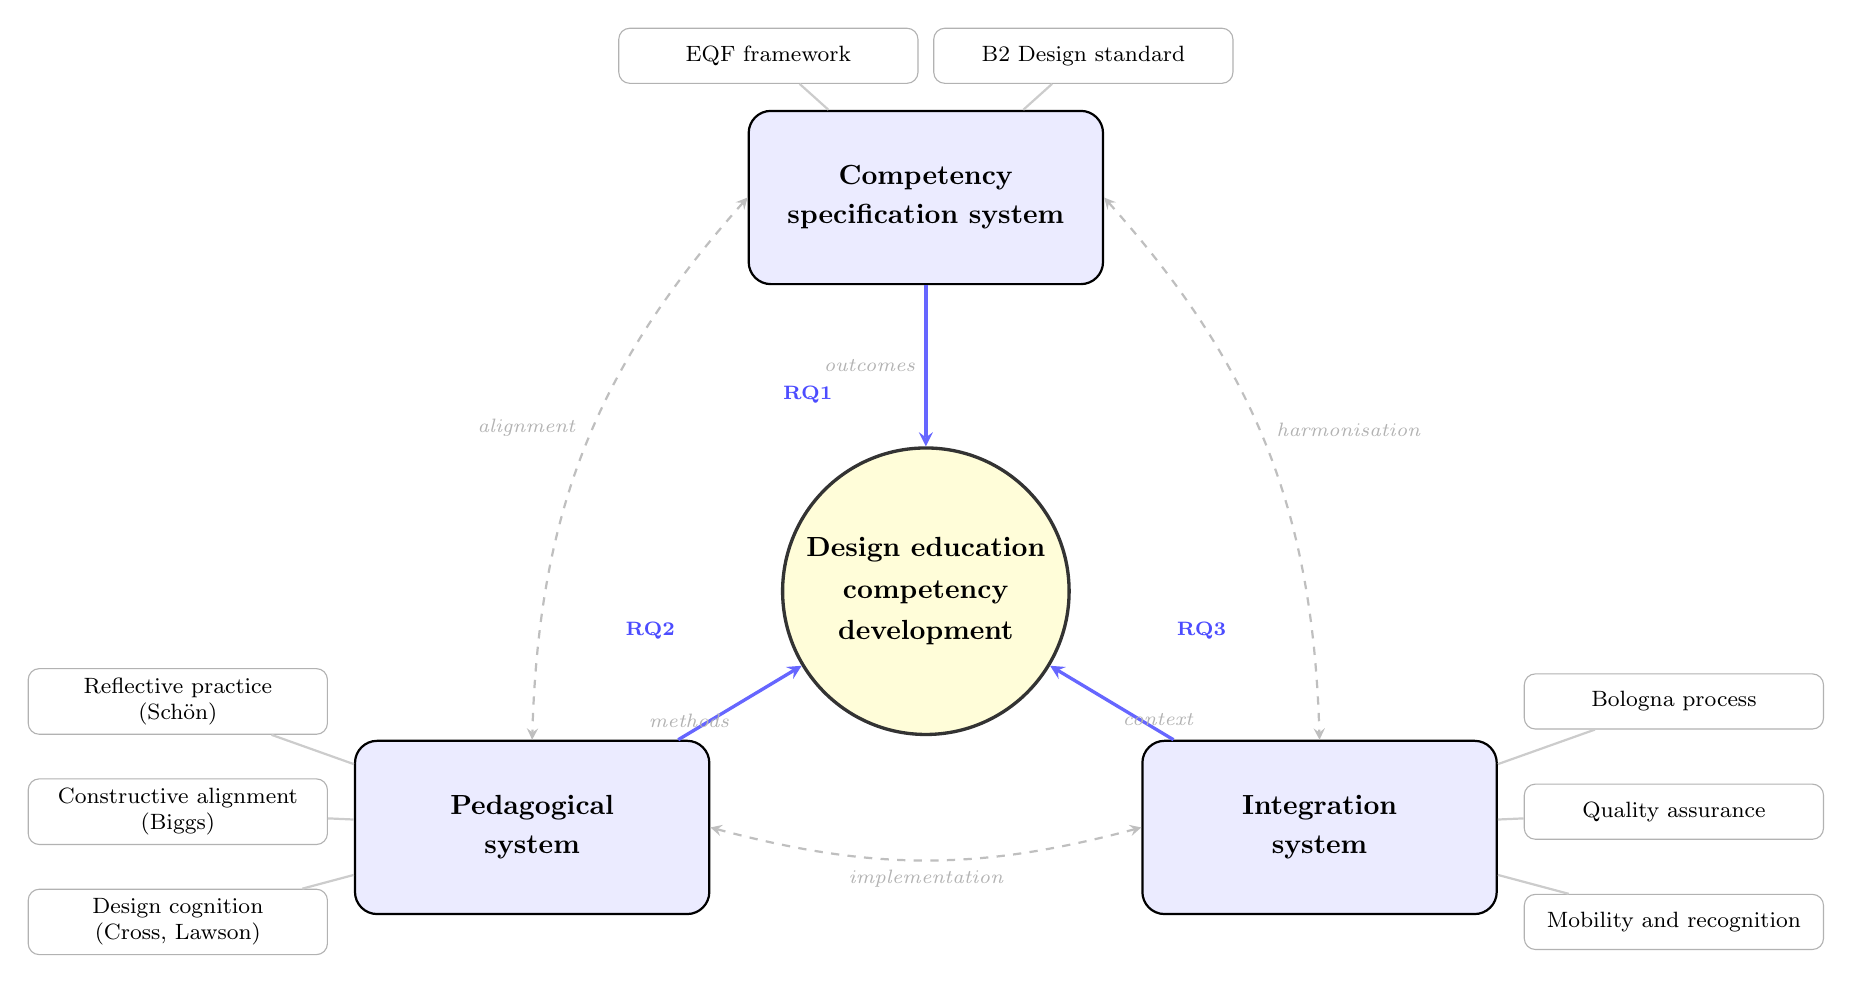
\begin{tikzpicture}[
				% Define styles
				corenode/.style={circle, draw=black!80, very thick, minimum size=3.2cm, align=center, fill=yellow!15},
				systembox/.style={rectangle, draw=black, thick, rounded corners=8pt, minimum width=4.5cm, minimum height=2.2cm, align=center, fill=blue!8},
				theorybox/.style={rectangle, draw=gray!60, rounded corners=4pt, minimum width=3.8cm, minimum height=0.7cm, align=center, fill=white, font=\footnotesize},
				processarrow/.style={->, very thick, >=stealth, draw=blue!60},
				feedbackarrow/.style={<->, thick, >=stealth, draw=gray!50, dashed},
				label/.style={font=\scriptsize\itshape, text=gray!60}
				]
				
				% Central core
				\node[corenode] (core) at (0,0) {\textbf{Design education}\\[3pt]\textbf{competency}\\[3pt]\textbf{development}};
				
				% Three system nodes
				\node[systembox] (competency) at (0,5) {\textbf{Competency}\\[2pt]\textbf{specification system}};
				\node[systembox] (pedagogy) at (-5,-3) {\textbf{Pedagogical}\\[2pt]\textbf{system}};
				\node[systembox] (integration) at (5,-3) {\textbf{Integration}\\[2pt]\textbf{system}};
				
				% Theory boxes for Competency System
				\node[theorybox] (eqf) at (-2,6.8) {EQF framework};
				\node[theorybox] (b2) at (2,6.8) {B2 Design standard};
				
				% Theory boxes for Pedagogical System
				\node[theorybox] (schon) at (-9.5,-1.4) {Reflective practice\\(Schön)};
				\node[theorybox] (biggs) at (-9.5,-2.8) {Constructive alignment\\(Biggs)};
				\node[theorybox] (design) at (-9.5,-4.2) {Design cognition\\(Cross, Lawson)};
				
				% Theory boxes for Integration System
				\node[theorybox] (bologna) at (9.5,-1.4) {Bologna process};
				\node[theorybox] (qa) at (9.5,-2.8) {Quality assurance};
				\node[theorybox] (mobility) at (9.5,-4.2) {Mobility and recognition};
				
				% Main arrows from systems to core
				\draw[processarrow] (competency) -- node[left, label] {outcomes} (core);
				\draw[processarrow] (pedagogy) -- node[below left, label] {methods} (core);
				\draw[processarrow] (integration) -- node[below right, label] {context} (core);
				
				% Theory box connections
				\draw[gray!40, thick] (eqf) -- (competency);
				\draw[gray!40, thick] (b2) -- (competency);
				\draw[gray!40, thick] (schon) -- (pedagogy);
				\draw[gray!40, thick] (biggs) -- (pedagogy);
				\draw[gray!40, thick] (design) -- (pedagogy);
				\draw[gray!40, thick] (bologna) -- (integration);
				\draw[gray!40, thick] (qa) -- (integration);
				\draw[gray!40, thick] (mobility) -- (integration);
				
				% Inter-system feedback loops
				\draw[feedbackarrow] (competency.west) to[bend right=20] node[above left, label] {alignment} (pedagogy.north);
				\draw[feedbackarrow] (competency.east) to[bend left=20] node[above right, label] {harmonisation} (integration.north);
				\draw[feedbackarrow] (pedagogy.east) to[bend right=15] node[below, label] {implementation} (integration.west);
				
				% Process labels
				\node[font=\scriptsize\bfseries, text=blue!70] at (-1.5,2.5) {RQ1};
				\node[font=\scriptsize\bfseries, text=blue!70] at (-3.5,-0.5) {RQ2};
				\node[font=\scriptsize\bfseries, text=blue!70] at (3.5,-0.5) {RQ3};
				
			\end{tikzpicture}
		}
		\caption{Integrative theoretical framework for design education competency development. The framework positions competency development at the intersection of three interacting systems, with research questions (RQ1--RQ3) addressing specific system relationships. Dashed arrows indicate feedback processes among systems.}
		\label{fig:theoretical-framework}
	\end{figure}
	
	The framework conceptualises competency development as an emergent property of system interactions rather than a linear product of any single system. The competency specification system establishes formal requirements through frameworks such as the EQF and national standards, including Ukraine's B2 Design. The pedagogical system encompasses the teaching and learning approaches~-- studio-based learning, project-based pedagogy, and reflective practice~-- through which competencies are developed. The integration system represents the broader policy environment of European harmonisation, quality assurance mechanisms, and recognition processes.
	
	Critically, the framework emphasises bidirectional relationships among systems, represented by dashed feedback arrows. Competency specifications influence pedagogical choices, but pedagogical traditions also shape how competencies are interpreted and operationalised. Integration requirements create pressures for standardisation, yet the distinctive nature of design education generates tensions with standardised approaches. These dynamic interactions constitute the analytical focus of the subsequent findings.
	
	\subsection{Application to research questions}
	
	The theoretical framework structures the analysis of each research question. RQ1, concerning alignment between the B2 Design standard and European frameworks, is addressed through examination of the competency specification system and its harmonisation relationship with the integration system. The analysis applies Biggs's constructive alignment principle to assess coherence between specified competencies and their intended outcomes.
	
	RQ2, concerning pedagogical approaches for the development of artistic-project competency, is addressed through the lens of pedagogical systems. Schön's reflective practice theory and Cross's design cognition research provide criteria for evaluating which pedagogical approaches offer the strongest theoretical grounding for design-specific competency development.
	
	RQ3, concerning European integration challenges and opportunities, is addressed through analysis of integration system dynamics and their interactions with both competency specification and pedagogical systems. The framework's emphasis on bidirectional relationships highlights how integration processes create both pressures and possibilities for reforming design education.
	
	\subsection{Framework limitations}
	
	The theoretical framework, while integrative, carries inherent limitations. As a synthesis of perspectives developed in different intellectual traditions, it risks conceptual tensions that require careful navigation. The constructive alignment principle, developed within outcomes-based education discourse, may not fully accommodate the open-ended, emergent nature of design learning that reflective practice theory emphasises. Similarly, design cognition research has focused primarily on professional practice rather than educational development, requiring extension to pedagogical contexts.
	
	Furthermore, the framework privileges cognitive and structural dimensions while giving less attention to social, cultural, and political factors that shape design education in specific national contexts. The Ukrainian case involves historical legacies, institutional cultures, and geopolitical circumstances that the framework acknowledges but does not fully theorise. These limitations are addressed through contextual sensitivity in the analysis while recognising the boundaries of the theoretical apparatus employed.
	
	% ==============================================================================
	% END OF THEORETICAL FRAMEWORK SECTION
	% ==============================================================================
	
	% Include Methodology
	% ==============================================================================
	% SECTION 5: METHODOLOGY
	% Design Education in Ukraine: Competency Development and European Integration
	% ==============================================================================
	
	\section{Methodology}
	\label{sec:methodology}
	
	This section presents the methodological approach employed in this theoretical study, detailing the research design, analytical procedures, and quality assurance measures. As a theoretical paper engaging in document analysis and conceptual synthesis, the methodology differs from empirical research designs while maintaining systematic rigour appropriate to scholarly inquiry.
	
	\subsection{Research design}
	
	This study employs a theoretical analysis approach combining document analysis with conceptual synthesis. Theoretical analysis, as a distinct methodological tradition, involves systematic examination of concepts, frameworks, and their interrelationships to develop new understanding or identify previously unrecognised connections \cite{Jaakkola2020}. Unlike empirical research that generates findings through data collection from participants or phenomena, theoretical analysis works with existing scholarly literature, policy documents, and conceptual frameworks as primary materials.
	
	The research design integrates two complementary analytical strategies. First, document analysis examines the Ukrainian B2 Design standard in conjunction with European competency frameworks, identifying both structural correspondences and divergences. Second, conceptual synthesis integrates international scholarship on design education, pedagogical theory, and competency-based education to develop an interpretive framework applicable to the Ukrainian context. Table~\ref{tab:research-design} summarises the research design elements.
	
	\begin{table}[htbp]
		\centering
		\caption{Research design summary.}
		\label{tab:research-design}
		\small
		\begin{tabularx}{\textwidth}{@{}lX@{}}
			\toprule
			\hfill \textbf{Design element} & \hfil \textbf{Specification} \\
			\midrule
			Research paradigm & Interpretivist; constructivist epistemology \\
			\addlinespace
			Research approach & Qualitative theoretical analysis \\
			\addlinespace
			Analytical strategies & Document analysis; conceptual synthesis \\
			\addlinespace
			Primary materials & Ukrainian B2 Design standard; EQF descriptors; Tuning project competencies; international design education scholarship \\
			\addlinespace
			Theoretical lenses & Reflective practice theory; constructive alignment; design cognition research \\
			\addlinespace
			Outputs & Integrative conceptual framework; comparative analysis; theoretical propositions \\
			\bottomrule
		\end{tabularx}
	\end{table}
	
	\subsection{Document selection and analysis}
	
	The document analysis component focuses on primary policy documents governing design education competencies. The central document is Ukraine's higher education standard for speciality B2 Design, approved by the Ministry of Education and Science in 2018 \cite{MON2018}. This standard specifies general competencies, professional competencies, and programme learning outcomes required for bachelor's degree programmes in design across Ukrainian higher education institutions.
	
	Comparative documents include the European Qualifications Framework level descriptors, particularly levels 6 and 7, which correspond to bachelor's and master's qualifications \cite{EuropeanCommission2017}. Additionally, the Tuning project competency frameworks provide disciplinary reference points developed through European collaboration \cite{Gonzalez2003}. These documents enable systematic comparison of competency structures across frameworks.
	
	The analytical procedure for document analysis follows established qualitative methods \cite{Bowen2009}. Initial reading establishes familiarity with document structure and terminology. Subsequent analytical reading identifies key competency categories, their definitions, and relationships among competency elements. Comparative analysis maps correspondences between Ukrainian and European frameworks, noting areas of alignment and divergence. Throughout this process, the theoretical framework guides interpretation, with particular attention to how competency specifications relate to pedagogical implications.
	
	\subsection{Literature synthesis procedure}
	
	The conceptual synthesis component draws on international scholarship identified through systematic literature searching. The search strategy employed multiple academic databases, including Scopus, Web of Science, and ERIC, using search terms combining design education, competency development, studio pedagogy, and European higher education. Searches were limited to peer-reviewed publications in English, with an emphasis on sources from 2015 to 2025 to capture contemporary developments, while also including foundational works from earlier periods.
	
	Literature selection prioritised sources addressing: (a) theoretical foundations of design education and design cognition; (b) pedagogical approaches in design disciplines, particularly studio-based and project-based learning; (c) competency-based education and European qualification frameworks; and (d) design education in European and post-Soviet contexts. Sources were evaluated for relevance to research questions, theoretical depth, and methodological quality.
	
	The synthesis procedure followed an integrative review methodology \cite{Torraco2005}, moving beyond summary toward critical analysis and conceptual development. Initial coding identified key themes and concepts across sources. Subsequent analysis examined relationships among concepts, identifying convergences, tensions, and gaps. The theoretical framework provided an organising structure for synthesis, with findings organised around the three systems (competency specification, pedagogical, and integration) and their interactions.
	
	\subsection{Analytical framework application}
	
	The theoretical framework presented in section~\ref {sec:framework} structures the analysis across three dimensions that correspond to the research questions. Figure~\ref{fig:methodology-process} illustrates the analytical process.
	
	\begin{figure}[htbp]
		\centering
		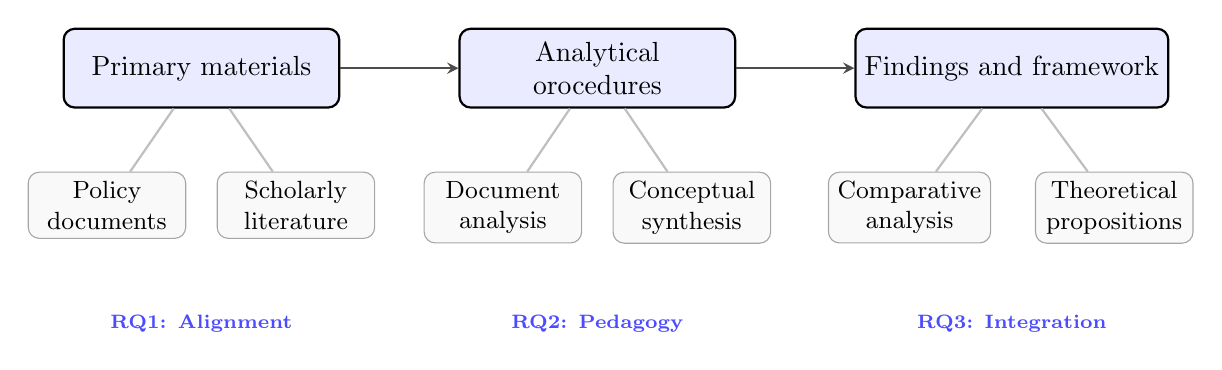
\begin{tikzpicture}[
			node distance=1.8cm,
			box/.style={rectangle, draw=black, thick, rounded corners, minimum width=3.5cm, minimum height=1cm, align=center, fill=blue!8},
			process/.style={rectangle, draw=gray!70, rounded corners, minimum width=2cm, minimum height=0.8cm, align=center, fill=gray!5, font=\small},
			arrow/.style={->, thick, >=stealth, draw=black!70},
			label/.style={font=\scriptsize, text=gray!60}
			]
			
			% Main flow - horizontal
			\node[box] (input) {Primary materials};
			\node[box, right=1.5cm of input] (analysis) {Analytical\\orocedures};
			\node[box, right=1.5cm of analysis] (output) {Findings and framework};
			
			% Process nodes below
			\node[process, below=0.8cm of input, xshift=-1.2cm] (doc) {Policy \\documents};
			\node[process, below=0.8cm of input, xshift=1.2cm] (lit) {Scholarly \\literature};
			
			\node[process, below=0.8cm of analysis, xshift=-1.2cm] (docana) {Document \\analysis};
			\node[process, below=0.8cm of analysis, xshift=1.2cm] (consyn) {Conceptual \\synthesis};
			
			\node[process, below=0.8cm of output, xshift=-1.3cm] (comp) {Comparative \\analysis};
			\node[process, below=0.8cm of output, xshift=1.3cm] (prop) {Theoretical \\propositions};
			
			% Main arrows
			\draw[arrow] (input) -- (analysis);
			\draw[arrow] (analysis) -- (output);
			
			% Vertical connections
			\draw[gray!50, thick] (doc) -- (input);
			\draw[gray!50, thick] (lit) -- (input);
			\draw[gray!50, thick] (docana) -- (analysis);
			\draw[gray!50, thick] (consyn) -- (analysis);
			\draw[gray!50, thick] (comp) -- (output);
			\draw[gray!50, thick] (prop) -- (output);
			
			% RQ labels
			\node[font=\scriptsize\bfseries, text=blue!70, below=2.5cm of input] {RQ1: Alignment};
			\node[font=\scriptsize\bfseries, text=blue!70, below=2.5cm of analysis] {RQ2: Pedagogy};
			\node[font=\scriptsize\bfseries, text=blue!70, below=2.5cm of output] {RQ3: Integration};
			
		\end{tikzpicture}
		\caption{Methodology process -- from primary materials through analytical procedures to findings and framework development, with research questions guiding each analytical dimension.}
		\label{fig:methodology-process}
	\end{figure}
	
	For RQ1 (competency alignment), the analysis compares competency categories and descriptors between the B2 Design standard and European frameworks. The comparison identifies: structural correspondences (similar competency categories), terminological variations (different language for similar concepts), and substantive gaps (competencies present in one framework but absent or underdeveloped in another).
	
	For RQ2 (pedagogical approaches), the analysis synthesises literature on design pedagogy, applying reflective practice theory and design cognition research as evaluative lenses. The synthesis identifies which pedagogical approaches offer the strongest theoretical grounding for developing the competencies specified in design education standards.
	
	For RQ3 (integration challenges), the analysis examines interactions among competency specification, pedagogy, and integration systems. Drawing on both document analysis and literature synthesis, the analysis identifies tensions, opportunities, and considerations relevant to the European integration trajectory of Ukrainian design education.
	
	\subsection{Quality assurance}
	
	Theoretical research requires quality assurance measures appropriate to its methodology. This study addresses trustworthiness through several strategies. Credibility is supported through the triangulation of multiple document sources and scholarly perspectives, ensuring that findings are not dependent on a single source. The theoretical framework provides an explicit analytical structure, enabling readers to follow interpretive logic.
	
	Transferability is addressed through thick description of the Ukrainian context and explicit articulation of the theoretical framework's assumptions and boundaries. While findings are context-specific, the analytical approach and conceptual framework may inform similar analyses in comparable contexts.
	
	Dependability is supported through systematic documentation of analytical procedures. The methodology section provides sufficient detail for readers to understand how conclusions were reached. Confirmability is addressed by grounding interpretations in documented sources, with citations that enable verification of claims.
	
	\subsection{Limitations}
	
	Several methodological limitations warrant acknowledgement. As a theoretical study, findings represent conceptual analysis rather than empirical validation. The propositions developed require subsequent empirical testing through research engaging design education stakeholders, curriculum implementation, and student outcomes.
	
	The document analysis relies on official policy documents, which may not fully reflect the realities of implementation. Standards and frameworks establish intentions; actual practice may diverge in ways not captured through document analysis alone. Additionally, the English-language focus of literature synthesis may underrepresent scholarship published in Ukrainian and other languages relevant to post-Soviet design education.
	
	%Finally, the author's positionality as external to Ukrainian institutional contexts shapes interpretive perspective. While external positioning enables comparative analysis, it may limit appreciation of contextual nuances familiar to those embedded in Ukrainian design education. These limitations are addressed through explicit acknowledgement and appropriate hedging of claims, while recognising that all research involves perspectival constraints.
	
	% ==============================================================================
	% END OF METHODOLOGY SECTION
	% ==============================================================================
	
	% Include Findings
	% ==============================================================================
	% SECTION 6: FINDINGS
	% Design Education in Ukraine: Competency Development and European Integration
	% ==============================================================================
	
	\section{Findings}
	\label{sec:findings}
	
	This section presents findings from the theoretical analysis, organised around the three research questions. The analysis examines the alignment of competencies between Ukrainian and European frameworks (RQ1), pedagogical approaches for developing artistic-project competency (RQ2), and European integration considerations for Ukrainian design education (RQ3).
	
	\subsection{RQ1: Competency framework alignment}
	
	The first research question investigated how the competency structures in Ukraine's B2 Design standard align with European qualification frameworks and international design education models. Document analysis reveals substantial structural alignment alongside significant conceptual variations, warranting attention.
	
	\subsubsection{Structural correspondences}
	
	The B2 Design standard demonstrates clear structural alignment with EQF architecture. The standard organises competencies into two categories~-- general competencies (ZK) and professional competencies (FK)~-- mirroring the EQF distinction between transversal and discipline-specific capabilities. Both frameworks position bachelor's-level qualifications at level 6, requiring demonstrated ability to apply knowledge in complex, unpredictable contexts with responsibility for decision-making.
	
	Table~\ref{tab:competency-alignment} presents the comparative alignment between B2 Design competencies and EQF level 6 descriptors across knowledge, skills, and responsibility/autonomy dimensions.
	
	\begin{table}[htbp]
		\centering
		\caption{Competency alignment: B2 Design standard and EQF Level 6.}
		\label{tab:competency-alignment}
		\small
		\begin{tabularx}{\textwidth}{@{}p{2.5cm}XXc@{}}
			\toprule
			\hfil \textbf{Dimension} & \hfil \textbf{EQF level 6 descriptor} & \hfil \textbf{B2 Design specification} & \textbf{Alignment} \\
			\midrule
			Knowledge & Advanced knowledge of a field of work or study, involving critical understanding of theories and principles & Knowledge of design history, theory, and methodology; understanding of artistic-project activity principles & Strong \\
			\addlinespace
			Skills & Advanced skills demonstrating mastery and innovation required to solve complex and unpredictable problems & Skills in artistic-project activity; ability to solve complex design problems with incomplete information & Strong \\
			\addlinespace
			Responsibility and autonomy & Manage complex technical or professional activities; take responsibility for decision-making & Ability to work independently and in teams; responsibility for professional development & Moderate \\
			\addlinespace
			Critical thinking & Implied in problem-solving and decision-making & General competency ZK1: critical thinking and analysis & Strong \\
			\addlinespace
			Communication & Implied in professional contexts & General competency ZK6: professional communication & Strong \\
			\bottomrule
		\end{tabularx}
	\end{table}
	
	The analysis identifies strong alignment in knowledge and skills dimensions, where both frameworks emphasise advanced, specialised capabilities applied to complex problems. The B2 Design standard's emphasis on artistic project activity as the integrating competency domain corresponds well with EQF expectations for discipline-specific mastery, as demonstrated through practical application.
	
	\subsubsection{Terminological and conceptual variations}
	
	Despite structural alignment, significant terminological variations exist that may complicate cross-framework interpretation. The B2 Design standard employs the concept of `artistic-project activity' (khudozhno-proektna diialnist) as the central organising principle for professional competencies. This concept, rooted in Soviet-era design education terminology, integrates artistic and technical dimensions in ways that lack direct equivalents in Western European frameworks.
	
	The EQF's tripartite structure (knowledge, skills, competence) differs from the B2 Design standard's binary organisation (general and professional competencies). While mappable, this structural difference reflects deeper conceptual variations. The EQF treats competence as a distinct category encompassing both responsibility and autonomy, whereas the B2 Design standard distributes these elements across the two competency categories.
	
	Furthermore, the B2 Design standard's professional competencies emphasise aesthetic and artistic dimensions more explicitly than typical EQF-aligned frameworks in technical disciplines. Competencies such as `ability to conduct aesthetic analysis' and `capacity for artistic-imaginative thinking' foreground creative capabilities that EQF descriptors address only implicitly through general references to innovation and problem-solving.
	
	\subsubsection{Identified gaps}
	
	The comparative analysis identifies three areas where the B2 Design standard shows less developed alignment with contemporary international design education models:
	
	\begin{enumerate}
		\item 
		\textit{Critical reflection competencies.} While the B2 Design standard includes critical thinking as a general competency, explicit attention to reflective practice~-- the systematic reflection on one's own design process and decisions~-- appears underdeveloped compared to international models that foreground metacognitive capabilities \cite{Schon1983, Hameed2023310}.
		
		\item 
		\textit{Interdisciplinary collaboration.} Contemporary design increasingly operates at intersections with engineering, business, social sciences, and other fields \cite{Davis202397}. The B2 Design standard addresses teamwork generally but provides limited specification of interdisciplinary collaboration competencies, which are increasingly central to design practice.
		
		\item 
		\textit{Sustainability and social responsibility.} International design education discourse increasingly emphasises sustainable design and social responsibility as core competencies \cite{Maia2022105}. The B2 Design standard's competency specifications give limited explicit attention to these dimensions, though they may be addressed within programme-level implementation.
	\end{enumerate}
	
	\subsection{RQ2: Pedagogical approaches for competency development}
	
	The second research question examined which pedagogical approaches offer the strongest theoretical foundation for developing artistic project competencies in design students. The analysis synthesises design education scholarship through the theoretical lenses of reflective practice, constructive alignment, and design cognition.
	
	\subsubsection{Studio-based learning as foundation}
	
	The literature synthesis confirms that studio-based learning is the pedagogical approach with the strongest theoretical grounding for design competency development. Studio pedagogy aligns with multiple theoretical perspectives supporting its effectiveness:
	
	From a reflective practice perspective, the design studio creates conditions for reflection-in-action, as identified by \citet{Schon1983} as central to the development of professional expertise. The iterative cycle of designing, receiving feedback, and revising enables students to develop tacit knowledge through experiential engagement rather than relying solely on abstract instruction \cite{Mewburn2012363}.
	
	From a design cognition perspective, studio environments support the co-evolution of problem and solution characteristics that are characteristic of expert design thinking \cite{Cross2011}. Unlike instructional approaches that separate problem definition from solution generation, studio projects enable students to develop problems and solutions simultaneously, building cognitive patterns aligned with professional practice \cite{Lawson2005}.
	
	From a constructive alignment perspective, studio-based assessment through project critique enables direct evaluation of design competencies as demonstrated through design artefacts and process documentation. This alignment between learning activities (designing) and assessment (evaluating designs) supports coherent competency development \cite{Biggs1996}.
	
	\subsubsection{Complementary pedagogical approaches}
	
	While studio-based learning provides the foundation, the analysis identifies complementary approaches that strengthen specific competency dimensions:
	
	\begin{itemize}
		\item 
		
		\textit{Project-based learning with authentic briefs} extends studio pedagogy by situating design challenges within realistic professional contexts \cite{Kamalipour2022}. Authentic projects develop competencies in client communication, constraint negotiation, and professional responsibility that studio exercises with artificial briefs may not fully address.
		
		\item 
		
		\textit{Structured reflective practice} addresses the metacognitive dimensions identified as underdeveloped in many design programmes. Explicit instruction in reflection, supported by tools such as design journals and process portfolios, can develop the critical reflection competencies that distinguish expert practitioners \cite{Hameed2023310}.
		
		\item 
		
		\textit{Interdisciplinary collaborative projects} develop the collaboration competencies increasingly required in professional practice. Projects requiring engagement with students from other disciplines~-- engineering, business, social sciences~-- build competencies in cross-disciplinary communication and integration \cite{Chon2019187}.
	\end{itemize}
	
	Table~\ref{tab:pedagogy-competency} maps pedagogical approaches to specific competency development outcomes.
	
	\begin{table}[htbp]
		\centering
		\caption{Pedagogical approaches mapped to competency development.}
		\label{tab:pedagogy-competency}
		\small
		\begin{tabularx}{\textwidth}{@{}lXp{3.2cm}@{}}
			\toprule
			\hfill \textbf{Pedagogical approach} & \hfil \textbf{Primary competencies developed} & \hfil \textbf{Theoretical basis} \\
			\midrule
			Studio-based learning & Artistic-project activity; design process skills; aesthetic judgement; technical execution & Reflective practice; design cognition \\
			\addlinespace
			Project-based learning & Problem-solving; professional communication; constraint management; iterative development & Experiential learning; constructive alignment \\
			\addlinespace
			Structured reflection & Critical thinking; metacognition; self-assessment; professional identity & Reflective practice; metacognitive theory \\
			\addlinespace
			Collaborative projects & Teamwork; interdisciplinary communication; negotiation; integration skills & Situated learning; social constructivism \\
			\addlinespace
			Design research methods & Analytical capabilities; evidence-based design; user understanding; systematic inquiry & Design cognition; research methodology \\
			\bottomrule
		\end{tabularx}
	\end{table}
	
	\subsubsection{Pedagogical implications for B2 Design implementation}
	
	The analysis suggests that effective implementation of B2 Design competencies requires pedagogical approaches that:
	
	\begin{enumerate}
		\item Maintain studio-based learning as the core pedagogical environment while ensuring adequate resources (space, faculty ratios, materials) for effective studio instruction.
		\item Integrate structured reflective practice through explicit instruction and assessment of metacognitive competencies, addressing the gap identified in competency specifications.
		\item Incorporate authentic project experiences connecting academic work to professional contexts, developing professional responsibility and communication competencies.
		\item Create opportunities for interdisciplinary collaboration, preparing students for the cross-disciplinary nature of contemporary design practice.
	\end{enumerate}
	
	\subsection{RQ3: European integration considerations}
	
	The third research question examined conceptual considerations emerging from the analysis of European integration challenges and opportunities for Ukrainian design education. The findings reveal tensions that require navigation alongside opportunities for improvement.
	
	\subsubsection{Challenges and tensions}
	
	The integration of Ukrainian design education into European qualification frameworks generates several significant tensions that require careful navigation and management. European qualification frameworks emphasise standardised learning outcomes amenable to cross-national comparison and recognition, yet design education inherently values originality and creative divergence that resist standardisation \cite{Weldon2009168}. Ukrainian design education must therefore satisfy framework requirements without constraining the creative exploration essential to design learning.
	
	A related challenge concerns the relationship between explicit and tacit knowledge. Competency frameworks require the explicit articulation of learning outcomes for transparency and assessment; yet, design expertise substantially involves tacit knowledge~-- embodied capabilities, aesthetic sensibilities, and intuitive judgements~-- that resists complete explication \cite{Schon1983}. Developing assessment approaches that capture tacit competencies within framework requirements remains an ongoing methodological challenge.
	
	The tension between international harmonisation and national traditions presents additional complexity. The Bologna Process harmonisation facilitates mobility and recognition, but may also pressure convergence toward dominant European models. Ukrainian design education has distinctive traditions~-- namely, the integration of fine arts and applied arts training, an emphasis on drawing and craft skills, and a particular aesthetic orientation~-- that merit preservation even as it pursues European integration.
	
	Finally, resource constraints present practical obstacles to alignment. Effective design education requires substantial resources, including dedicated studio spaces, low student-faculty ratios for individual critique, and materials and equipment for prototyping. European integration expectations may exceed resource availability in Ukrainian institutions, particularly given ongoing disruptions.
	
	\subsubsection{Opportunities and possibilities}
	
	Framework alignment with European qualification structures also presents significant opportunities for Ukrainian design education. Enhanced mobility and recognition represent primary benefits, as alignment facilitates the movement of students and faculty within the European Higher Education Area. Ukrainian design students may access exchange opportunities, while international students may consider Ukrainian programmes, enriching educational experiences and building professional networks across national boundaries.
	
	Quality assurance enhancement provides another avenue for growth and development. European quality assurance mechanisms provide frameworks for systematic programme evaluation and improvement, and engagement with these mechanisms can strengthen Ukrainian design education through structured self-assessment and external review processes.
	
	Access to curriculum development resources constitutes a further advantage of European integration. European networks offer access to expertise in curriculum development, pedagogical innovations, and collaborative opportunities. Ukrainian institutions can draw on European experience while contributing distinctive perspectives from their own traditions, creating reciprocal knowledge exchange rather than unidirectional transfer.
	
	Ultimately, aligning with European competency frameworks may enhance labour market preparedness for Ukrainian design graduates. Increased competitiveness in European labour markets expands professional opportunities for individual graduates while contributing more broadly to economic development through the integration of Ukrainian creative industries within European markets.
	
	\subsubsection{Framework for navigation}
	
	Based on the analysis, figure~\ref{fig:integration-framework} presents a conceptual framework for navigating European integration in design education.
	
	\begin{figure}[htbp]
		\centering
		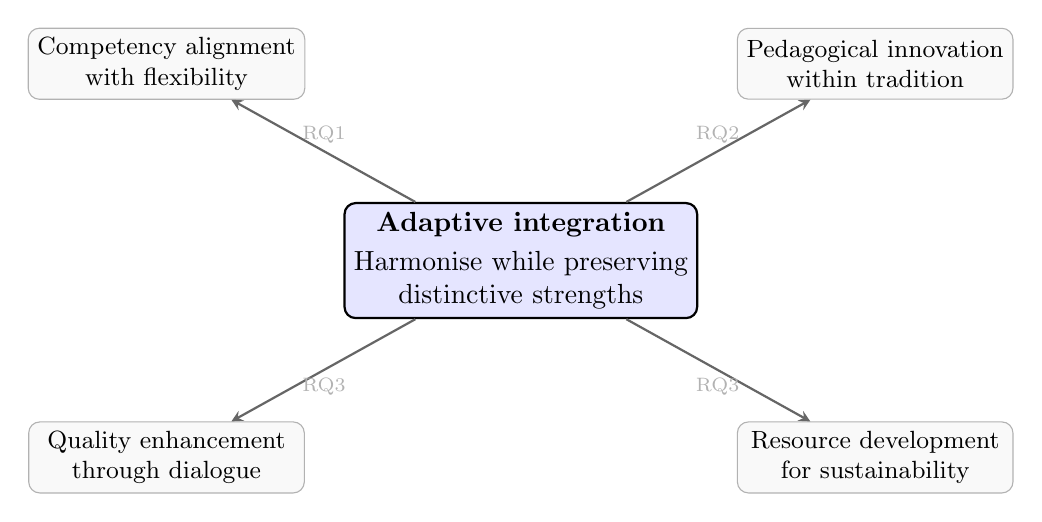
\begin{tikzpicture}[
			node distance=1.5cm,
			principle/.style={rectangle, draw=black, thick, rounded corners, minimum width=4cm, minimum height=1.2cm, align=center, fill=blue!10},
			strategy/.style={rectangle, draw=gray!60, rounded corners, minimum width=3.5cm, minimum height=0.9cm, align=center, fill=gray!5, font=\small},
			arrow/.style={->, thick, >=stealth, draw=black!60}
			]
			
			% Core principle
			\node[principle] (core) at (0,0) {\textbf{Adaptive integration}\\[2pt]Harmonise while preserving\\distinctive strengths};
			
			% Four strategic directions
			\node[strategy] (s1) at (-4.5,2.5) {Competency alignment\\with flexibility};
			\node[strategy] (s2) at (4.5,2.5) {Pedagogical innovation\\within tradition};
			\node[strategy] (s3) at (-4.5,-2.5) {Quality enhancement\\through dialogue};
			\node[strategy] (s4) at (4.5,-2.5) {Resource development\\for sustainability};
			
			% Arrows
			\draw[arrow] (core) -- (s1);
			\draw[arrow] (core) -- (s2);
			\draw[arrow] (core) -- (s3);
			\draw[arrow] (core) -- (s4);
			
			% Labels
			\node[font=\scriptsize, text=gray!60] at (-2.5,1.6) {RQ1};
			\node[font=\scriptsize, text=gray!60] at (2.5,1.6) {RQ2};
			\node[font=\scriptsize, text=gray!60] at (-2.5,-1.6) {RQ3};
			\node[font=\scriptsize, text=gray!60] at (2.5,-1.6) {RQ3};
			
		\end{tikzpicture}
		\caption{Conceptual framework for navigating European integration in Ukrainian design education -- adaptive integration as core principle with four strategic directions.}
		\label{fig:integration-framework}
	\end{figure}
	
	The framework positions `adaptive integration' as the guiding principle~-- pursuing European harmonisation while preserving and developing the distinctive strengths of Ukrainian design education. Four strategic directions operationalise this principle:
	
	\begin{enumerate}
		\item \textit{Competency alignment with flexibility} requires ensuring that B2 Design competencies map clearly to the EQF while maintaining space for programme-level adaptation and distinctive emphases.
		\item \textit{Pedagogical innovation within tradition} involves adopting effective pedagogical approaches from international practice while building on the strengths of Ukrainian design education traditions.
		\item \textit{Quality enhancement through dialogue} entails engaging European quality assurance as a developmental opportunity rather than a compliance burden, contributing Ukrainian perspectives to European discourse.
		\item \textit{Resource development for sustainability} demands addressing resource requirements strategically, leveraging European partnerships and funding opportunities while building sustainable institutional capacity.
	\end{enumerate}
	% ==============================================================================
	% END OF FINDINGS SECTION
	% ==============================================================================
	% Include Discussion
	% ==============================================================================
	% SECTION 7: DISCUSSION
	% Design Education in Ukraine: Competency Development and European Integration
	% ==============================================================================
	
	\section{Discussion}
	\label{sec:discussion}
	
	This section interprets the findings in relation to existing scholarship, develops implications for theory and practice, and articulates the contributions of this theoretical analysis. The discussion synthesises insights across the three research questions while acknowledging the limitations and boundaries of the analysis.
	
	\subsection{Interpretation of findings}
	
	The findings reveal a complex picture of Ukrainian design education's relationship to European frameworks~-- one characterised by substantial structural alignment alongside significant conceptual and practical challenges. This pattern reflects broader tensions in competency-based education reform across creative disciplines.
	
	\subsubsection{Competency frameworks: alignment and divergence}
	
	The strong structural alignment between the B2 Design standard and EQF confirms that Ukrainian policymakers have successfully adapted the European framework architecture to the national context. This alignment facilitates the formal requirements of European integration: credential recognition, credit transfer, and qualification comparability. However, the analysis reveals that structural alignment does not guarantee conceptual equivalence.
	
	The distinctive concept of `artistic-project activity' illustrates this tension. Rooted in Soviet-era traditions that integrated fine arts training with applied design, this concept organises professional competencies in ways that resist straightforward mapping to Western European frameworks. Rather than viewing this as a deficiency requiring correction, the analysis suggests it represents a distinctive strength~-- an integrative understanding of design competence that synthesises aesthetic and technical dimensions. This interpretation aligns with \citeauthor{Cross2011}'s \cite{Cross2011} argument that design constitutes a distinct cognitive domain irreducible to either art or engineering.
	
	The identified gaps~-- critical reflection, interdisciplinary collaboration, and sustainability~-- align with broader critiques of competency-based education in creative fields. \citet{Weldon2009168} notes the difficulty of capturing creative capabilities within standardised frameworks, while \citet{Brockmann200899} questions whether performance-based outcomes can adequately represent professional expertise. These concerns suggest that gaps in the B2 Design standard may reflect inherent limitations of competency frameworks rather than oversights in standard development.
	
	\subsubsection{Pedagogical foundations: studio pedagogy and beyond}
	
	The confirmation of studio-based learning as the foundational pedagogy for design competency development aligns with established scholarship \cite{Schon1983, Goldschmidt2010285}. However, the analysis extends this understanding by articulating specific mechanisms through which studio pedagogy develops different competency dimensions. The integration of reflective practice theory, design cognition research, and constructive alignment provides a multi-theoretic foundation that strengthens pedagogical justification.
	
	The identified need for complementary approaches~-- structured reflection, authentic projects, and interdisciplinary collaboration~-- suggests that studio pedagogy alone may be insufficient for developing the full range of competencies contemporary design practice requires. This finding resonates with \citeauthor{Davis202397}'s argument that design education must evolve beyond twentieth-century models focused on artefact production toward approaches that address complex socio-technical systems.
	
	Importantly, the analysis suggests that pedagogical enhancement need not abandon established traditions. Ukrainian design education's emphasis on drawing, craft skills, and artistic fundamentals represents accumulated pedagogical wisdom that should inform rather than impede innovation. The challenge involves integration rather than replacement~-- augmenting traditional strengths with approaches that address emerging competency requirements.
	
	\subsubsection{European integration: adaptive approaches}
	
	The framework of `adaptive integration' emerging from the analysis offers a conceptual alternative to polarised positions that either embrace uncritical harmonisation or resist European engagement defensively. Adaptive integration acknowledges the legitimate interests served by European frameworks~-- mobility, recognition, and quality assurance~-- while insisting on space for distinctive national and disciplinary traditions.
	
	This approach aligns with scholarship questioning whether European higher education policy adequately accommodates disciplinary diversity \cite{Bohlinger2012279}. Design education's distinctive features~-- the centrality of tacit knowledge, the value placed on creative originality, the integration of aesthetic and technical judgement~-- create tensions with frameworks developed primarily for more codifiable disciplines. Adaptive integration navigates these tensions through selective adoption rather than wholesale compliance.
	
	\subsection{Theoretical implications}
	
	The analysis contributes to theoretical understanding in several ways. First, it extends the application of reflective practice theory to competency-based curriculum development. While \citet{Schon1983} developed the concept primarily to understand professional expertise, this analysis applies it evaluatively~-- using reflective practice as a criterion for assessing pedagogical approaches and competency specifications. This extension suggests productive connections between practice-based professional education theory and the development of policy-oriented competency frameworks.
	
	Second, the integrative theoretical framework demonstrates how multiple theoretical perspectives can be synthesised for design education analysis. Rather than privileging single theories, the framework positions reflective practice, constructive alignment, and design cognition as complementary lenses illuminating different dimensions of design education. This synthetic approach may inform future research that seeks a multidimensional understanding of design learning.
	
	Third, the concept of adaptive integration contributes to theorising educational reform in contexts of regional integration. Existing scholarship tends toward either celebration of harmonisation benefits or critique of standardisation pressures. Adaptive integration offers a middle position that acknowledges both dimensions while providing conceptual resources for navigation.
	
	\subsection{Practical implications}
	
	The findings generate several practical implications for different stakeholders. Table~\ref{tab:implications} summarises key implications for curriculum developers, educators, policymakers, and researchers.
	
	\begin{table}[b]
		\centering
		\caption{Practical implications for design education stakeholders.}
		\label{tab:implications}
		\small
		\begin{tabularx}{\textwidth}{@{}lX@{}}
			\toprule
			\hfill\textbf{Stakeholder} & \hfil\textbf{Key implications} \\
			\midrule
			Curriculum developers & Address identified competency gaps (critical reflection, interdisciplinary collaboration, sustainability) through explicit learning outcomes and assessment criteria; maintain studio-based learning as core while integrating complementary approaches; preserve distinctive strengths of Ukrainian design education tradition \\
			\addlinespace
			Design educators & Integrate structured reflective practice into studio instruction; develop assessment approaches capturing tacit competencies; create opportunities for authentic project experiences and interdisciplinary collaboration; balance technological innovation with foundational skill development \\
			\addlinespace
			Policymakers & Support resource development for effective studio instruction (space, materials, faculty ratios); facilitate European partnerships while protecting curricular autonomy; develop quality assurance approaches appropriate to creative disciplines; invest in faculty development for contemporary pedagogies \\
			\addlinespace
			Researchers & Conduct empirical research validating theoretical propositions; investigate implementation of B2 Design standard across institutions; examine stakeholder perspectives on European integration; develop assessment instruments for design competencies \\
			\bottomrule
		\end{tabularx}
	\end{table}
	
	For curriculum developers, the analysis provides both diagnostic insights (where gaps exist) and prescriptive guidance (how to address them). The emphasis on integration rather than replacement suggests that curriculum revision should build on existing strengths while strategically addressing identified limitations.
	
	For educators, the multi-theoretic pedagogical foundation offers conceptual resources for understanding and improving practice. The specific mechanisms linking pedagogical approaches to competency development provide actionable guidance for instructional design.
	
	For policymakers, the adaptive integration framework suggests approaches to European engagement that satisfy harmonisation requirements while preserving distinctive national traditions. The resource implications~-- particularly for studio-based instruction~-- highlight investment priorities.
	
	\subsection{Limitations and future directions}
	
	Several limitations constrain the scope and applicability of these findings. As a theoretical analysis, the study develops conceptual propositions rather than empirically validated conclusions. The alignment assessment, pedagogical recommendations, and integration framework require empirical testing through research engaging actual curriculum implementation, stakeholder perspectives, and student outcomes.
	
	The document analysis focused on official standards and frameworks, which may not fully reflect the realities of implementation. Institutional practices often diverge from policy intentions in ways that document analysis cannot capture. Future research should examine how the B2 Design standard is interpreted and implemented across different institutional contexts.
	
	The English-language focus of the literature synthesis may underrepresent relevant scholarship in Ukrainian and other languages. Post-Soviet design education has developed substantial scholarly traditions that merit inclusion in comprehensive analyses of the field.
	
	Future research directions emerging from this analysis include:
	
	\begin{itemize}
		\item Empirical studies of B2 Design standard implementation across Ukrainian institutions, examining variation in interpretation and resource allocation.
		\item Comparative research examining design education reform in other post-Soviet countries engaging European integration.
		\item Stakeholder research investigating how design educators, students, and employers perceive competency frameworks and integration processes.
		\item Assessment development research creating instruments appropriate for evaluating design competencies, particularly tacit and creative dimensions.
		\item Longitudinal research tracking graduate outcomes to assess relationships between competency-based education and professional success.
	\end{itemize}
	
	\subsection{Contribution summary}
	
	This theoretical analysis contributes to design education scholarship in three principal ways. First, it provides a systematic analysis of Ukrainian design education standards in relation to European frameworks, addressing a gap in English-language scholarship on post-Soviet design education. Second, it develops an integrative theoretical framework that synthesises reflective practice, constructive alignment, and design cognition perspectives for the analysis of design education. Third, it articulates the concept of adaptive integration as an approach to European harmonisation that balances standardisation pressures with preservation of distinctive traditions.
	
	These contributions extend understanding of design education reform while offering conceptual resources applicable beyond the Ukrainian case. As design education globally confronts pressures for standardisation alongside demands for creativity and innovation, frameworks for navigating these tensions become increasingly valuable.
	
	% ==============================================================================
	% END OF DISCUSSION SECTION
	% ==============================================================================
	% Include Conclusion
	% ==============================================================================
	% SECTION 8: CONCLUSION
	% Design Education in Ukraine: Competency Development and European Integration
	% ==============================================================================
	
	\section{Conclusion}
	\label{sec:conclusion}
	
	This theoretical analysis has examined Ukrainian design education through the lens of competency development and European integration, addressing three interrelated research questions concerning framework alignment, pedagogical approaches, and integration considerations. The analysis contributes to understanding design education reform in contexts of transition while offering conceptual resources applicable to similar cases internationally.
	
	\subsection{Summary of key findings}
	
	The analysis reveals that Ukraine's B2 Design standard demonstrates strong structural alignment with the European Qualifications Framework architecture, facilitating formal recognition and mobility requirements. However, significant conceptual variations exist, particularly regarding the distinctive Ukrainian concept of `artistic-project activity' that integrates aesthetic and technical dimensions in ways without direct Western European equivalents. Three competency gaps warrant attention: critical reflection capabilities, interdisciplinary collaboration skills, and sustainability-oriented competencies.
	
	Regarding pedagogical approaches, the analysis confirms studio-based learning as the foundational pedagogy for design competency development, supported by convergent theoretical perspectives from reflective practice, design cognition, and constructive alignment. Complementary approaches~-- structured reflection, authentic project experiences, and interdisciplinary collaboration~-- address competency dimensions that studio pedagogy alone may not fully develop.
	
	The European integration analysis identifies four principal tensions requiring navigation: standardisation versus creativity, explicit versus tacit knowledge articulation, international harmonisation versus national traditions, and resource constraints versus quality requirements. Correspondingly, four opportunities emerge: enhanced mobility and recognition, quality assurance development, curriculum resources through European networks, and improved labour market preparation.
	
	\subsection{Conceptual contributions}
	
	This study makes three principal contributions to the scholarship of design education. First, it provides a systematic English-language analysis of Ukrainian design education standards, addressing a geographical gap in international scholarship on post-Soviet design education. This analysis enables comparative understanding while making Ukrainian developments accessible to international audiences.
	
	Second, the integrative theoretical framework synthesising reflective practice theory, constructive alignment, and design cognition research offers a multi-dimensional analytical apparatus for design education analysis. This framework demonstrates how complementary theoretical perspectives can illuminate different dimensions of competency development while maintaining a coherent analytical structure.
	
	Third, the concept of adaptive integration provides conceptual resources for navigating European harmonisation processes. By positioning harmonisation and tradition preservation as compatible rather than contradictory goals, adaptive integration offers an alternative to polarised positions that either embrace uncritical convergence or resist engagement defensively.
	
	\subsection{Recommendations}
	
	Based on the analysis, the following recommendations emerge for Ukrainian design education development:
	
	\begin{enumerate}
		\item Competency framework refinement requires addressing identified gaps through explicit articulation of critical reflection, interdisciplinary collaboration, and sustainability competencies within programme-level learning outcomes, while preserving the distinctive strengths of the artistic-project activity orientation.
		
		\item Pedagogical enhancement involves maintaining studio-based learning as the core pedagogical environment while systematically integrating structured reflective practice, authentic project experiences, and interdisciplinary collaborative opportunities.
		
		\item Resource investment necessitates prioritising resources essential for effective design education—dedicated studio spaces, appropriate student-faculty ratios, materials and equipment—recognising that quality design education requires sustained investment.
		
		\item European engagement entails pursuing European partnerships strategically, leveraging opportunities for mobility, quality assurance development, and curriculum innovation, while maintaining curricular autonomy that is appropriate to distinctive national and disciplinary traditions.
		
		\item Research development demands conducting empirical research examining B2 Design standard implementation, stakeholder perspectives, and graduate outcomes to validate theoretical propositions and inform evidence-based policy development.
	\end{enumerate}
	
	\subsection{Concluding reflections}
	
	Design education globally confronts a paradox: the same qualities that make design valuable~-- creativity, innovation, and the capacity to envision alternatives~-- resist the standardisation that contemporary educational governance demands. Ukrainian design education navigates this paradox within the additional complexity of European integration and ongoing national challenges.
	
	The adaptive integration framework developed in this analysis suggests that this paradox need not be paralysing. Harmonisation and distinctiveness can coexist when integration is approached strategically rather than mechanically. European frameworks provide valuable architecture for articulating and recognising competencies; Ukrainian design education traditions provide rich pedagogical resources for developing them. The task involves synthesis rather than substitution.
	
	As design increasingly addresses complex socio-technical challenges that require creativity, collaboration, and systemic thinking, the competencies developed through effective design education become increasingly valuable. Ukrainian design education, drawing on its distinctive traditions while engaging with international developments, has the potential to make a meaningful contribution to this global endeavour. This analysis provides conceptual resources that support this contribution.
	
	% ==============================================================================
	% END OF CONCLUSION SECTION
	% ==============================================================================
	% ==============================================================================
	% GENERATIVE AI DECLARATION
	% ==============================================================================
	\begin{aideclaration}
		This paper was developed with the assistance of Claude (Anthropic). This large language model was utilised for the following purposes: developing literature search strategies, revising manuscript sections, formatting and compiling LaTeX documents, managing BibTeX references, and creating TikZ diagrams. The author critically evaluated, verified, and revised all AI-generated content to ensure accuracy, appropriateness, and alignment with the research objectives. The author assumes full responsibility for the final content, analysis, interpretations, and conclusions presented in this work. %The use of generative AI is disclosed in accordance with emerging standards for transparency in academic publishing.
	\end{aideclaration}
	
	% Bibliography
	\bibliography{references}
	
\end{document}